\chapter{Research Methodology and Data}

This chapter focuses on describing which approaches were chosen for the task at hand and why, as well as shows how the work progressed. 

To reiterate the current problem is to find out if \gls{gnn} can compete at solving the \gls{mwm} problem compared to other approximation methods such as greedy algorithm.

\section{Challenges}

It is common to think of a neural network as of a black box where you give some data to this box and it tries to predict the correct answer. In this case the data is a graph consisting of vertices connected by edges that have weights and the expected answer should be pairs of vertices that were matched together.

As mentioned the idea behind supervised learning is to give a model the correct answers so it can by trial and error learn from it. Theese answers are not included in the initial datasets so the optimal solutions needs to be calculated. To find the optimal solution Blossom algorithm implemented by Joris van Rantwijk in Python was used \cite{mwmBlossom}. This does however point out an important weakness of the supervised approach. Obviously a model needs to be able to handle graphs of different sizes and it is the large ones that are most interesting. Finding an optimal for algorithmic problems for the large graphs can be time consuming, at the same time a model need as much data as possible to learn, leading to multiple large graphs consuming to much time combined. This poses a question whether it is possible for the model to learn on small and medium sized graphs that are not as time consuming and transfer learned patterns to solve larger graphs.

Another important aspect that must be taken in to the consideration is that it is unlikely for the model to fully follow the restictions of the problem. Model might decide to match same node to 2 neighbors at the same time, which should not be allowed. 

\section{Main Idea}

To summarize, given a weighted udirected graph, the \gls{nn} must predict  a valid subset of edges or in other words pairs of vertices that maximize the total weight. The \gls{nn} will have a graph as an input and the otput will be the probabilities (0.00 - 1.00) of how likely an edge will be in the matching. To control that a solution is valid, instead of picking all the edges with the probability higher than 50\%, the edges can be sorted by their probabilities and greedily picked in that order if they don't break the validity of the solution. This might sound illogical to use greedy algorithm on the models output to beat the normal greedy algorithm with weights, but the fact that edges are now sorted not by their weight, but a score decided by \gls{nn} does make a difference, since the \gls{gnn} can take multiple features in consideration when assigning probabilities. Some of these features come naturaly such as structure of the graph, and some we can manualy add during preprocessing. 

\gls{nn}s have a lot of hyperparameters and methods that can be tuned to make a model better suited for the task. The ideal way of finding the best combination of the hyperparameters is to try as many combinations as possible. Train a model for each combination and choose the one with best performance. This is a time consuming procedure however and therefore in this task the exploration of hyperparameters was narrowed down to the ones that seemed most important and indicated positive impact during early experiments. 

During the experiments following hyperparameters were tested:
\begin{enumerate}
\item Learning rate - by how much the weights of the model should be corrected
\item Network depth and width - layers and neurons
\item Class weights - how much should the model focus on a given class. Classes being: 
	\begin{itemize}
	\item 0 = is NOT in the solution.
	\item 1 = is in the solution.
	\end{itemize}	
\item Weight decay - used to keep \gls{gnn} weight values relatively small and decrease chances of the model memorizing the answers. 

\item Additionally other methods were tried such as augmenting data (adding extra features to the nodes during preproccessing): 
	\begin{itemize}
	\item Degree - how many neighbours a node has
	\item Weight relative to the sum of neighbours.
	\item Weight difference from the sum of the neighbours.
	\item Sums of the weights. 
	\item 1st largest weight, 2nd largest weight.
	\end{itemize}

\end{enumerate}

\section{Data}

The model should be capable of solving any graph relevant to \gls{mwm} problem. A relevant graph can be difined by following characterisitcs
Ideally the model should be able to handle any kind of an udirected graph with weighted edges.

For training and experimenting with the \gls{gnn}, a MNIST dataset was used \cite{dwivedi2022benchmarking}. The dataset consists of 70000 relatively small graphs with 70 nodes and 564 edges on average. Graphs also include features for the edges representing distances between node. Theese features is what is used as the weights for the problem. Although the graphs in this dataset are relatively small they have some fitting qualities such and nodes having many neighbors creating more possible ways to match the nodes. Small size also makes it less time consuming to train the models and try different approaches as well as shows whether a \gls{gnn} trained on smaller graphs can transfer its knowledge to larger graphs.

Only training and testing on MNIST graphs does not represent all the different graphs that can occur, therefore model had to be tested on other graphs that have different structures and weight distributions. Model trained exclusively on MNIST dataset did not perform well on other graphs as one might ha expected. Therefore another dataset was made to cover larger variety of graphs. The dataset was a collection of random graphs from SuitSparse database that ranged between 100 and 10000 nodes. As described in more details in the \hyperref[sec:preprocessing]{Data preprocessing section}, some of the found graphs did not have edge weights. In these cases random weights were generated.

Including truly large graphs in training caused problems with insufficient memory and too long training time, but final model was still tested on some larger graphs than used in training. A couple large graphs from SuiteSparse were chosen for testing performance on large graphs with 40000 nodes and higher.

Small handcrafted graphs were used to test if \gls{gnn} can at least beat the cases specificaly made to abuse weaknesses of a greedy approach.

\section{Architecture}
\label{sec:architecture}
During the experiments the architecture of the \gls{gnn} model itself had mostly minor changes, but 2 rather different graph preproccessing steps were tried. In both cases we use \gls{gcn} layers (GCNConv) \cite{gcnpaper}. The GCNConv layer fits well for the purpose of this task because it makes use of the edge weights that are the crucial part for solving \gls{mwm}.

Python example:
\begin{lstlisting}[language=Python]
class MyGCN(torch.nn.Module):
    def __init__(self):
        super().__init__()
        self.conv1 = GCNConv(5, 640) # 5 features per each node, initialy 1
        self.conv2 = GCNConv(640, 640)
        self.lin = Linear(640, 2) # 2 classes 
\end{lstlisting}

For training, Adam optimizer was used \cite{kingma2017adam}. Optimizer is used to adjust the weights of the network during training. Adam optimizer has several hyperparameters that can be usefull to achieve better results and is one of the popular optimizers to use.

Now, let us go through the whole process of a graph being matched using the \gls{gnn} presented here.

\subsection{Model pipeline}

As mentioned before one cannot fully trust the model to satisfy the restrictions of the problem. What is meant by the restrictions of the probem is the fact that every node can only be matched once. This is controlled by sorting the probabilities the model's outputs in descending order and adding matches to the final solution one by one, skipping matches that already have matched nodes. Another potential problem can happen at the end when some of the nodes that can be matched were not matched at all by the model. There is a chance of that happening, since only pick the matches with high enough probability are used. As a starting point probability threshold is 50\% and above. Two things are done to ensure nothing is left to waste. First, after the model is done the potential remainder of the graph is fed to the model again. For model this would essentialy just be a new graph and it may happen that model manages to match the remainder given the new context. This process can be repeated several times and the break condition is if 0 matches were made in the last iteration. At that point if anything is left, which hopefully is a small fraction of the initial graph, can be solved using standard greedy or any other approximation algorithm for that matter.

Passing the graph and it's consecutive remainders multiple times through the model can also be helpfull to deal with the case where one of the matches that was picked may play big role in how the rest of the solution will look like. Idealy to handle this case one might only pick one match at the time and pass the graph through the model again, but it will be too time consuming.

\subsection{Line Graph Approach}

Line graph approach was the first attempt at using a simple \gls{gnn}, which later turned out to be too time consuming for larger graphs to be worth further expriements. It did however give some usefull insight as well as a showed to be a proof of concept. In the context of graphs line graph is a complement of the original graph that turns each edge to a vertex and connects the vertices if they shared a vertex in the original graph. 

Examaple of a graph and its line graph convertion
\begin{figure}[H]
    \centering
    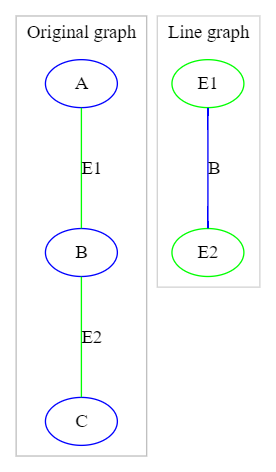
\includegraphics[scale=0.5]{figures/LineGraphExample}
    \caption{Original graph (left) and its line graph (right)}
    \label{Line graph figure}
\end{figure}

Converting to a line graph makes the architecture of the \gls{gnn} model simpler. Instead of needing to ask model for each pair of nodes is they should be matched together, the line graph model now can output the probability of a node being in the matching directly, since the node now represents two connected nodes from original graph. This also however transforms the problem itself. From the perspective og the model it is now trying to solve \gls{mwis}. \gls{gnn}s for \gls{mis} have been studied before. Nouranizadeh et. al. showed demonstrated a pooling method for solving \gls{mwis} \cite{DBLPjournals/corr/abs-2107-01410}. Unfortunately the large graphs can explode in size when converted to line graphs and were too time consuming in such cases.

\subsection{Edge Classification Approach}

A more natural way of approaching this problem is to give the model original graphs instead of transforming them to line graphs. But the model itselv only returns some numerical representation on the nodes in the graph. To get the predictions for the edges one can add a classifier module to the existing \gls{gnn}. This module's purpuse is to predict if a pair of two nodes will be in the matching. So the first part of the model produces embedding for each node and then for each edge, embeddings of both nodes are put together and passed to the classifier. Resulting in the model output being probabilities of all the edges being in the matching.

Python example:

\begin{lstlisting}[language=Python]

class MyGCNEdge(torch.nn.Module):
    def __init__(self):
        super().__init__()
        self.conv1 = GCNConv(7, 640)
        self.conv2 = GCNConv(640, 640)
        self.embed = Linear(1280, 80)

class EdgeClassifier(torch.nn.Module):
    def __init__(self):
        super().__init__()
        self.lin1 = Linear(160, 320) # 80 * 2 features since input is 2 nodes.
        self.lin2 = Linear(320, 2)

    def embedEdges(self, nodeEmbed, graph):
        x_src, x_dst = nodeEmbed[graph.edge_index[0]], nodeEmbed[graph.edge_index[1]]
        edgeEmbed = torch.cat([x_src, x_dst], dim=-1)        
        return edgeEmbed

\end{lstlisting}

\subsection{Data preprocessing}
\label{sec:preprocessing}
Not all graphs found in the database are fit for the training as is, and the ones that fit perfectly are few. Machine learning models require some preproccessing of data before it can be used. Convertion to the line graph is one example of such preproccessing. One might also need to augment the initial data to improve model performance. Finally machine learning models can be vulnerable to large numerical swings in the data, such as edge weights being higher than expected.

Most important are the edge weights. To ensure we have enough graphs to train on and the graphs cover a variety of structures, some of the chosen graphs that lacked weights recieved a randomly generated weights. The random weights had even distribution in the range between 0 and 1. All the graphs with preexisting weights were also adjusted to be in that range by shifting the weights to positive range if any negative weights were detected and then dividing by the largest weight. The weights could have been in any range, but the important thing is to have consistent weights for all the graphs. 

Another preprocessing step that was added is additional features for the nodes/vertices. This required different approaches for line graph and edge prediction approaches since in a line graph vertex represents an edge from the original graph. Line graph has weights assigned to the nodes themselves while using original graph nodes are assigned to edges.

One vertex feature does reamain in common: Degree of the nodes. Meaning how many neighbors each node has.

Line garphs node features:  

\begin{enumerate}
\item Weight relative to the sum of neighbours. For each vertex v:  \[ Wrel = v.weight  \div  (\sum_{n=0}^{|neighbors|} neighbors[n].weight) \]
\item Weight difference from the sum of the neighbours. For each vertex v:  \[ Wdiff = v.weight  \div  (\sum_{n=0}^{|neighbors|} neighbors[n].weight) \]
\item Sums of the neighbouring node weights. \[ (\sum_{n=0}^{|neighbors|} neighbors[n].weight) \]
\end{enumerate}

Normal graph edge features. Here some adjustments are made since nodes do not have any weights assigned unlike line graph.

\begin{enumerate}
\item Sum of the weights of all the outgoing edges.  \[ Wsum = (\sum_{i=0}^{|edges|} edges[i].weight) \]
\item Wsum relative to the Wsum of neighbours. For each vertex v:  \[ Wrel = Wsum \div (\sum_{n=0}^{|neighbors|} neighbors[n].Wsum) \]
\item Wsum difference from the Wsum of the neighbours. For each vertex v: \[ Wdiff = Wsum \div (\sum_{n=0}^{|neighbors|} neighbors[n].Wsum) \]
\end{enumerate}

\section{Result Validation}

Before looking at the results it is important to decide how to evalueate results properly and what is important for the problem at hand:

\begin{enumerate}
\item Time - how long an algorithm took to produce an answer. For the \gls{gnn} this includes model specific preproccessing such as adding additional features as well as finishing the potential remainder of the graph with greedy algorithm.
\item Correctness - is the answer correct. In case of \gls{mwm} the total weight aquired would be the measurement of how correct the solution is. It is unlikely that \gls{gnn} can find an optimal solution for more complex problems so it is reasonable to look at how close \gls{gnn} comes to the optimal solution.
\item GNN portion - due to the way program is set up, if the model does not match the whole graph, the rest of the graph will need to be finished somehow. This is done by running normal greedy algorithm at the end if anything is left. Because of that there can be cases where the model does nothing and by default achieves 100\% result of what normal greedy algorithm would. Therefore the portion of the weights obtained directly by the model needs to be evaluated as well.
\end{enumerate}

\subsection{Sanity checks}

It can often happen that during the project something goes wrong with the model and it can be not obvious. Therefore, one often does what is called sanity checks to see if model's inputs and outputs still make sense. 

Following "sanity checks" were done:
	\begin{enumerate}

\item To ensure the model and data are functioning correctly we trained a model on a small dataset for a long enough time and tested it on the same data. The model should be able to memorize theese graphs and solve the problem near perfect on them.

\item Comparisons to random matching were done. Before the training the model has random weights and essentialy will behave as if it is picking edges at random, but after training the model was performing better than a random matching.

\item The model was tested on a small hand crafted graphs that were made specificaly to put greedy algorithm in disadvantage. That at least showed that the model goes in the right direction even if it only manages to solve the easy cases.
	\end{enumerate}	

\section{Expected Results}

\subsection{Accuracy and total weight}

There are not that many researches specifically for \gls{mwm}, but problems like \gls{mis} that are relatively close to \gls{mwm} can indicate similar results for this case as well. As discussed in the \hyperref[sec:background]{Background section}, there are researches that show that \gls{gnn}s are capable of solving \gls{co} problems and beating greedy algorithms, while other rather indicate that improvements are still needed for it to be worth using. Therefore it is hard to forecast any results based on previous work. Nothing stands in the way of being optimistic however, additionally to the fact that greedy algorithm is relatively simple and \gls{nn} should be able the recognise a more complex pattern it can use to achieve better results. It is absolutely not expected for the model to be able to find optimal solution since any \gls{nn} is a heuristic. The margin by which \gls{gnn} can surpass the greedy solution is expected to be rather small, since from the data analysis it was abserved that for the majority of graphs greedy algorithm preforms rather well with above 80\% of the optimal possible weight.

\subsection{Time}

\gls{gnn} model is a heuristic solver and gives an approximate answer. Therefore model should be noticeably faster than exact algorithm, otherwise it would not be worth it. The time a model takes to solve one instance of a problem should be closer to that of a greedy algorithm and probably slightly longer due to preproccessing required such as augmenting data with adittional features. Naturaly, time will also depend on the depth and the width of the network.

\subsection{Remainder or model portion}

Ideally the model should be able to handle the full graph on its own, but as long as the model manages to improve final result it would still be a usefull tool. A speculative estimation for the sake of having something for orientation will be 80\%. That is the weight obtained from models prediction makes at least 80\% of total weight.

\subsection{Other observations}

One improtant observation was made during the analysis of the data that is worth mentioning. The difference between the optimal solution and the greedy is in most cases is rather small. For the MNIST dataset and the majority of the graphs found on Suite Sparse Matrix Collection the greedy algorithm manages to reach 90+\% of the optimal weight. Assigning random evenly distributed values to the edges weights also seem to give the same results. For the \gls{gnn} this means that it will be rather difficult to beat the greedy algorithm since it gets very close to the optimal.
